% !TeX root = ../main.tex

\chapter{机器学习}
\label{cha:ML}

LHC上的ATLAS实验接收质子-质子对撞事例的速率约为$1kHz$,每个事例所占的内存大小约为$1.3MB$,这些原始的对撞数据将会被用作后续的粒子重建、校准、分析等工作~\cite{PERF-2007-01}。
而这个大型实验装置的目标主要分为两类,第一个标准模型的精确测量,第二是寻找超出标准模型的新物理,无论哪个目标都要求我们在如此庞大的数据体系中将所需要的信号和本底提取和区分开来。
这就使得机器学习~\cite{RevModPhys.91.045002}能作为一种非常有用的技术手段被应用到高能物理实验(HEP)领域中来,机器学习旨在在大量数据的基础上降低数据的复杂性和发现数据中新的特征,
最早是在十九世纪末二十世纪初,一部分物理学家将简单的前馈神经网络用于事例分类,
而后慢慢的由决策树代替~\cite{JNN62,JNN63,JNN64},这样长达十年之久,从2014年开始,随着深度学习的崛起,
物理学家发现它应用在事例分类等方面相比之前的效果有了显著的提升~\cite{JNN65,JNN66},Baldi等人在2014年将深度学习神经网络第一次用在事例筛选,
用于标定超出标准模型的新粒子,结合MC模拟发现它不仅优于决策树,而且不需要那些精心设计过的事例变量作为输入~\cite{JNN67},
紧接着,他们又引入了参数化的分类器~\cite{JNN68},随后深度学习神经网络接连被用于jet的标定~\cite{JNN69,JNN70,JNN71}和jet味信息的标定~\cite{JNN72},
而且,依赖各种不同的物理模型,不同模式的深度学习神经网络也发展了起来~\cite{JNN73,JNN74,JNN75,JNN76},
除了与jet相关的方面,机器学习在高能物理实验的其他方面都有了比较成功的应用,比如说事例和粒子鉴定、能量分析和堆积事例压低等~\cite{Albertsson_2018}。
而当前高能物理实验领域使用最广的两种机器学习算法是深度学习神经网络(DNN)和提升决策树(BDT),本章将对它们做个概述,读者可以参考书目~\cite{MLTsinghua,MLMIT}详细了解。


\section{神经网络}
\label{sec:NN}

神经网络是一种一般性的多元函数$f:	\mathbb{R}^N\rightarrow\mathbb{R}^M$,将一个代表输入特征的向量$\boldsymbol{x}=(x_1,x_2,	\dots,x_N)$映射到一个有代表性的输出向量$\boldsymbol{y}=(y_1,y_2,	\dots,y_M)$。
这种映射通常可以被用于分类或者回归问题。如图~\ref{fig:BP}所示,这类多元函数是通过用一系列称之为隐层(hidden layers)的结构将输入层$\boldsymbol{x}$(input layers)和输出层$\boldsymbol{y}$(output layers)连接而构建起来的。

\begin{figure}  
  \begin{center}
    \begin{subfigure}{.9\textwidth}
     \centering
    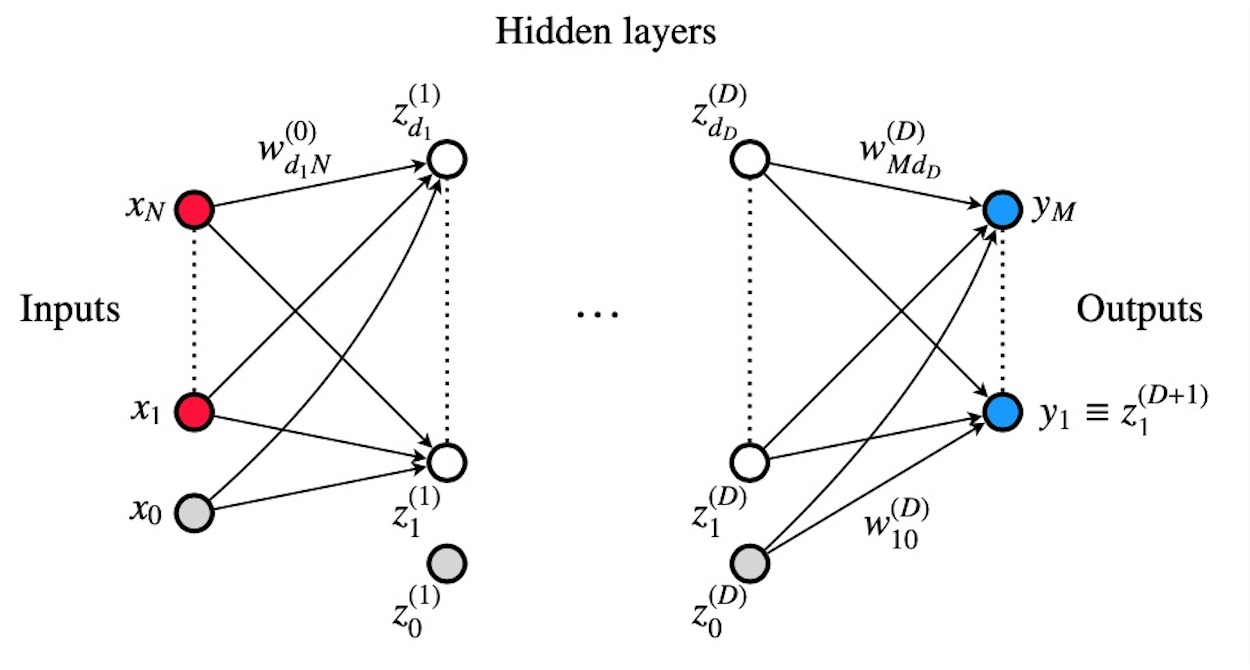
\includegraphics[width=0.75\textwidth]{figuresML/FP.jpg}
    \caption{正向传播过程}
    \end{subfigure}
    \begin{subfigure}{.9\textwidth}
     \centering
    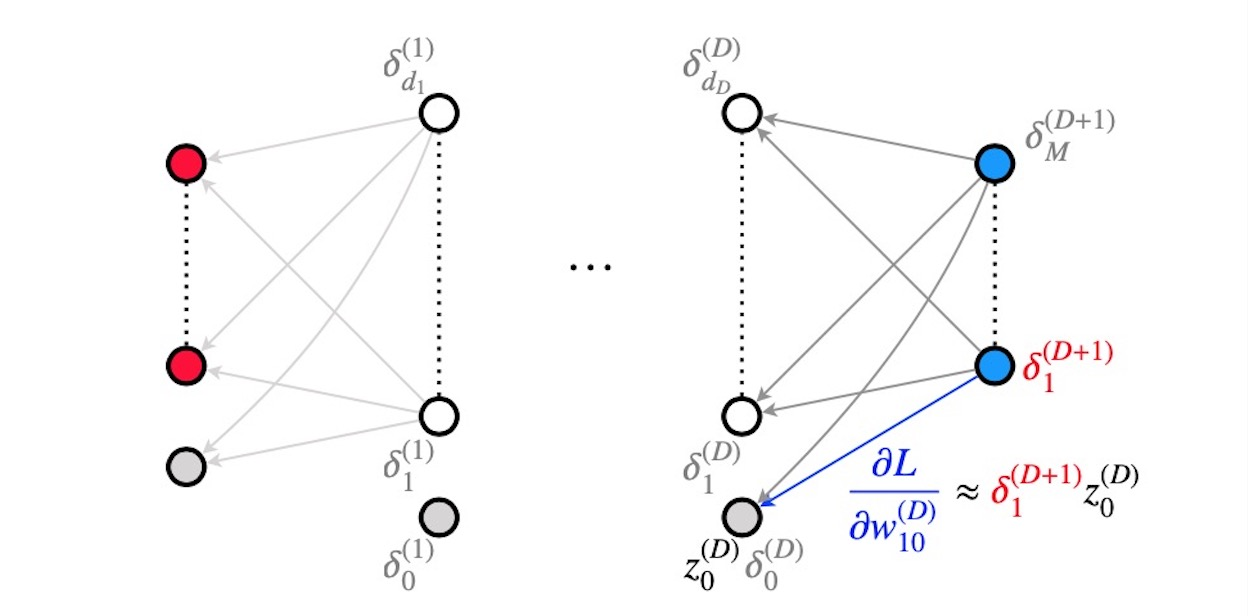
\includegraphics[width=0.75\textwidth]{figuresML/BP.jpg}
    \caption{反向传播过程}
    \end{subfigure}
  \end{center}
  \caption{
前馈(feed-forward)的密集连接型(densely connected)神经网络~\cite{FDNN}示意图。每个节点代表一个输入或者输出,每条线代表一个权重因子。反向传播算法的学习过程由(a)和(b)两个过程组成。
  }
  \label{fig:BP}
\end{figure}

相邻层之间的连接是通过一个线性变换和一个非线性的激活函数$h:\mathbb{R}^N\rightarrow\mathbb{R}^M$(activation function)实现的:
\begin{equation} 
\label{eq:ml1}	
a_{i}^{(l+1)}=\sum_{j=1}^{d_l} w_{ij}^{(l)}z_{j}^{(l)} + b_{i}^{(l)} = \sum_{j=0}^{d_l} w_{ij}^{(l)}z_{j}^{(l)}, \quad z_{i}^{(l)}=h(a_{i}^{(l)})
\end{equation}
其中,$l$是层指标,$\boldsymbol{z}^{(l)}={z_{i}^{(l)}}$是第$l$层中每个被称为节点(node)的值,$d_l=\|\boldsymbol{z}^{(l)}\|$是第$l$层中总的节点数目,$\boldsymbol{W}^{(l)}={w_{ij}^{(l)}}$是$d_{l+1} \times d_l$权重矩阵,
$\boldsymbol{b}^{(l)}={b_{i}^{(l)}}$是长度为$\|\boldsymbol{b}^{(l)}\|=d_{l+1}$的偏移向量,$\boldsymbol{a}^{(l)}={a_{i}^{(l)}}$是第$l$层中节点的线性组合或者输出,作为非线性激活函数的输入。输入和输出层分别对应于$\boldsymbol{x}=\boldsymbol{z}^{(0)}$和$\boldsymbol{y}=\boldsymbol{z}^{(D+1)}$。这里将神经网络的整个参数集记为$\theta$。

神经网络的体系结构是由隐层和每个隐层的节点配置所决定的,通常会被作为训练阶段的一部分得到优化。
每个附加的隐层和隐层中每个附加的节点都会为神经网络增加可调参数,从而增加神经网络的容量。这就使得神经网络能近似成任意复杂的连续函数。通常,神经网络也被称为通用型估计器(universal approximators),这意味着,在容量足够的情况下,它能以任意的精度近似成任意的连续函数~\cite{MLSV}。因此,在用于调整神经网络参数的数据集足够大的情况下,这个性质使得它非常适合复杂的计算任务。


\subsection{训练}
\label{sec:Train}

到此,我们介绍了神经网络的基础,其中信息流是以输入到输出的方式前向传播的。接着,比较关键的一个概念是对神经网络的训练,即针对一个特定的分类或者回归任务,调整网络的结构参数$\theta$,这便是机器学习中“学习”的过程。
在训练开始的时候,网络的结构参数$\theta$不是已知的,通常是从某个分布比如说高斯分布中随机取样进行初始化的。
在标准的$\chi^2$回归分析法~\cite{WENDT1991275}当中,可以精确的计算目标函数相对于每个拟合参数的梯度,从而可以使用一定的梯度下降算法来最小化目标函数。
然而对于神经网络,可能有数百万个结构参数,从而参数空间维数太大,使得上述方法不可行,因此需要一种新的方法来实现网络的结构参数调节。

与函数优化相似的是,神经网络的训练是通过最小化某个特定任务的目标函数,或者被称为损失函数(loss funcion)$L$来实现的。

对于回归任务,在给定输入集$X$和目标集$Y$的情况下,损失函数是均方差(MSE):
\begin{equation} 
\label{eq:ml2}	
L_{MSE}(\theta) = \mathbb{E}_{\boldsymbol{x} \sim X, \boldsymbol{y} \sim Y} \left[ \frac{1}{M} \sum_{i=1}^M (y_i - p_i (\boldsymbol{x} \mid \theta))^2 \right]
\end{equation}
其中$\mathbb{E}$表示一组相关联的输入集和回归目标的平均,$\theta$是神经网络的结构参数集,$p_i (\boldsymbol{x} \mid \theta)$是给定结构参数集$\theta$条件下神经网络对应于输入集$\boldsymbol{x}$的第$i$个预测输出。这个损失函数是神经网络的预测输出与相对应的回归目标之间的平均欧式距离。

对于带有关联标记$y\in\{[1,0,0],[0,1,0],[0,0,1]\}$的输入集$\boldsymbol{x}$的多分类任务,在神经网络的最后一层通常会使用\textsc{SoftMax}~\cite{MLMIT}作为激活函数,用以确保将神经网络的三个输出变量都限制在开区间$(0,1)$内。
这种情况下,可以使用多分类交叉熵(categorical cross-entropy,CCE)作为损失函数:
\begin{equation} 
\label{eq:ml3}	
L_{CCE}(\theta) = \mathbb{E}_{\boldsymbol{x} \sim X, \boldsymbol{y} \sim Y} \left[ - \sum_{i=1}^3 (y_i log p_i (\boldsymbol{x} \mid \theta)) \right]
\end{equation}
同样,这里$p(\boldsymbol{x} \mid \theta)$是给定结构参数集$\theta$条件下神经网络对应于输入集$\boldsymbol{x}$的预测输出。
此处的多分类交叉熵对应于体系的似然函数的对数的负数值,因此可以将其理解为在给定结构参数集$\theta$和输入集$\boldsymbol{x}$情况下标记$y$出现的概率~\cite{MLSV}。


\subsection{反向传播算法}
\label{sec:BackProp}

在根据式~\ref{eq:ml2}或~\ref{eq:ml3}中损失函数来训练神经网络时,由于参数空间维数太大,需要一种不依赖结构参数空间中每个参数独立变化的方法来估计梯度$\partial L / \partial w_{ij}^{(l)}$。
因为式~\ref{eq:ml1}中带有$D$个隐层的标准神经网络就是$D+1$个非线性可微函数的组合,那么,微积分中的链式法则可以被用来估计梯度,从而可以用近似梯度下降算法来训练神经网络。

在一个密集连接型神经网络~\cite{DenNet}中,式~\ref{eq:ml1}中$a^{(l-1)}$的变化是通过它们与$a^{(l)}$的连接而引起$L_{MSE}$或$L_{CCE}$的变化。如图~\ref{fig:BP},中间输出层$a^{(l)}$也直接依赖于第$l$层中的权重因子$w_{ij}^{(l-1)}$。由于神经网络中所有线性变换以及损失函数相对于线性变换中的权重都是可微的,因此可以在此处用到链式法则:
\begin{equation} 
\label{eq:BP1}	
\frac{\partial L}{\partial w_{ij}^{(l)}} \bigg\rvert_{\{\boldsymbol{x},\boldsymbol{y}\}} \equiv \frac{\partial L}{\partial w_{ij}^{(l)}} \equiv \underbrace{\frac{\partial L}{\partial a_{i}^{(l+1)}}}_{\equiv \delta_{i}^{(l+1)}} \frac{\partial a_{i}^{(l+1)}}{\partial w_{ij}^{(l)}} = \delta_{i}^{(l+1)}z_{j}^{(l)}
\end{equation}
其中$\delta_{i}^{(l+1)}$是为代替$\frac{\partial L}{\partial a_{i}^{(l+1)}}$而引入的缩写,称之为误差,右边第二项由式~\ref{eq:ml1}得到。
这就表示,损失函数相对于权重因子的梯度是由输入节点的值和这个权重因子所连接的误差决定的,如图~\ref{fig:BP}所示。
这种梯度计算方法和依赖关系适用于任意一组输入集$\boldsymbol{x}$和目标集$\boldsymbol{y}$。
为了方便起见,可以利用链式法则进一步对隐层中的误差进行分解:
\begin{equation} 
\label{eq:BP2}	
\delta_{i}^{(l)}=\frac{\partial L}{\partial a_{i}^{(l)}}=\sum_k \underbrace{\frac{\partial L}{\partial a_{k}^{(l+1)}}}_{= \delta_{k}^{(l+1)}} \underbrace{\frac{\partial a_{i}^{(l+1)}}{\partial a_{i}^{(l)}}}_{= w_{ki}^{(l)}h' \left( a_{i}^{(l)} \right) } \approx h' \left( a_{i}^{(l)} \right) \sum_k \delta_{k}^{(l+1)} w_{ki}^{(l)}
\end{equation}
这里再次用到了式~\ref{eq:BP1}中误差的定义和式~\ref{eq:ml1},其中$h'$是激活函数的一阶微分。式~\ref{eq:BP2}将第$l$层每个节点的误差和第$l+1$层节点的误差联系了起来。初始条件由含$D$个隐层的神经网络的输出层$l=D+1$的误差给出:
\begin{equation} 
\label{eq:BP3}	
\delta_{i}^{(D+1)}=\frac{\partial L}{\partial a_{i}^{(D+1)}}= \frac{\partial L}{\partial z_{i}^{(D+1)}} \frac{\partial z_{i}^{(D+1)}}{\partial a_{i}^{(D+1)}} = \frac{\partial L}{\partial p_{i}} h' \left( a_{i}^{(D+1)} \right)
\end{equation}
通过递归运用式~\ref{eq:BP3}可以将误差从输出层$l=D+1$反向传播到输入层$l=0$,
给定这些误差之后,损失函数相对于神经网络中各个权重因子的微分由式~\ref{eq:BP1}给出。
因此,对于每个输入集$\boldsymbol{x}$和对应的目标集$\boldsymbol{y}$,最简单的情况是通过以下方法更新神经网络中的权重,从而达到最小化损失函数的目的:
\begin{equation} 
\label{eq:BP4}	
w_{ij}^{(l)} \leftarrow w_{ij}^{(l)} - \eta \frac{\partial L}{\partial w_{ij}^{(l)}} \bigg\rvert_{\{\boldsymbol{x},\boldsymbol{y}\}} = w_{ij}^{(l)} - \eta \delta_{i}^{(l+1)}
\end{equation}
其中$\eta$是学习速率,用于控制每次权重更新的尺度,从而控制随机梯度下降(stochastic gradient descent)的速率。通过迭代权重更新式~\ref{eq:BP4},可以在训练神经网络时实现最小化损失函数$L(\theta)$。


\section{提升决策树}
\label{sec:BDT}

决策树(Decision tree, DT)~\cite{BDT2,BDT1}是另一种机器学习算法。
与神经网络类似,它可以将一个N维特征输入向量$\boldsymbol{x}=(x_1,x_2,	\dots,x_N)$映射到一个代表特征类的概率值或一个函数值,
这取决于具体任务是分类问题还是回归问题。
这里以二进制分类(binary classification)问题为例来具体说明。
为了构建二进制决策树,标准的分类和回归决策树算法(The standard classification and regression tree, CART)
通过在单个特征上进行二进制筛选来顺序划分输入特征空间。
首先,决策树从包含整个训练数据的单个节点开始,这个起始节点被称为根节点R,
在最简单的情况下,任务会对数据进行一次拆分,使得数据被最优地分为两个类,成为两个部分,
分类之后会出现两个子节点N,分别代表被分开的两部分。
为了找到最佳分类,算法会对每个特征输入$\boldsymbol{x}$进行扫描,
并根据代表具体任务的某些度量来评估该分割,一种常用的度量称为基尼指数~\cite{BDT1}。

在根节点进行第一次拆分之后,这个拆分过程会递归应用到每个子节点上面,
根据具体任务,每次拆分都会使得局部类纯度最大化。
这种顺序的二进制拆分会形成一个“二进制树”,
其中每个内部节点都对应一个特定的决策,因此被命名为“决策树”。
后续的每一步都是为了提高类纯度,
当训练数据中每个样本都被正确的归类或者达到某些停止条件的时候,
拆分便会停止,比如限制决策树的最大节点层数。
分类结束后,决策树的最后一层节点称为叶节点,
从根节点到叶节点的每条路径称为分支。
决策树中的这些属性便是其结构参数,会根据每个实际的任务得到优化。
图~\ref{fig:BDT}~展示的是一个简单的二进制决策树及其特征空间划分示例。

\begin{figure}
  \begin{center}
    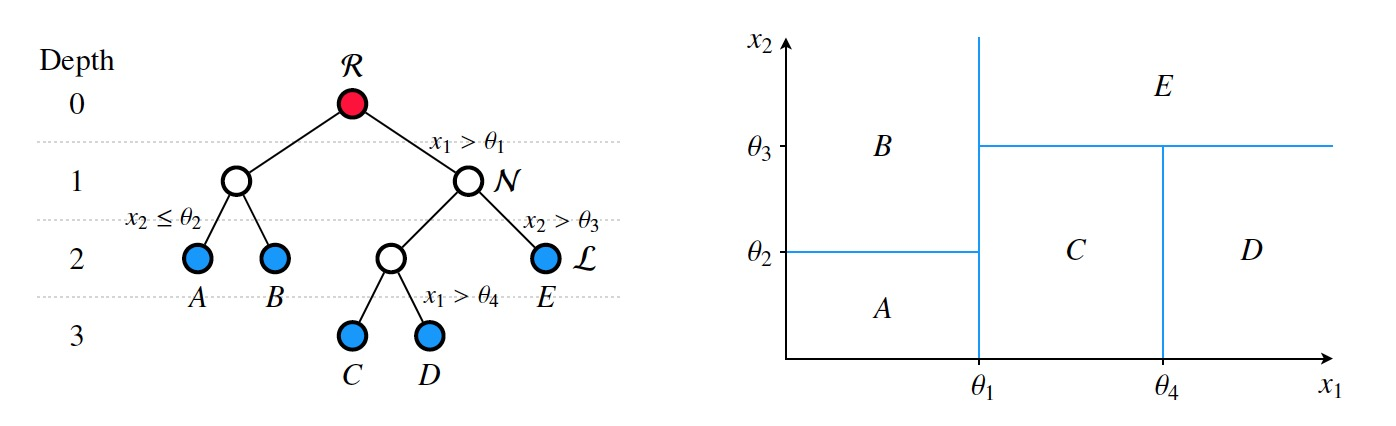
\includegraphics[width=0.9\textwidth]{figuresTHE/BDT.jpg}
  \end{center}
  \caption{二维特征输入$\boldsymbol{x}=(x_1,x_2)$的二进制决策树示例(左图),其中包含一个根节点、三个决策节点和五个叶节点将
  输入特征空间分为五个不相交的决策区间(右图)。 }
    \label{fig:BDT}
\end{figure}

在单个决策树中,每个叶节点表示的特征子空间内的样本将具有相同的预测输出值,
对于分类问题,预测值是叶节点上每个相同类上的训练样本所占的比例,
而对于回归问题,预测值是目标函数的平均值。
从这里可以看出决策树的决策功能不连续,
这对于大多数关系都是连续的高能物理领域来说是不理想的,
于是在此基础上引入了称为提升的方法。
该方法的出发点是通过组合一系列较弱的学习本领而得到一个较强的学习本领,

提升决策树(Boosted decision trees, BDT)~\cite{BDT3,BDT4}算法会按顺序训练一系列的决策树,记为提升梯级t。
在每个提升梯级中,分配给在上一梯级中修改过的每个训练样本的权重都会增加,
从而增加它的重要性。
然后根据提升梯级中t中错误分类的训练样本的加权比例来计算一个决策树权重$a^t$,
最后通过加权平均将所有的决策树组合在一起:
\begin{equation} 
\label{eq:BDT}
BDT(\boldsymbol{x})=\sum_t a^t DT^t(x) 	
\end{equation}
通过这种决策树的提升方法,可以得到一个更强大的提升决策树算法,
它能为样本进行更好的分类,而且不容易过拟合,也不会像单个决策树那样出现决策不连续的问题。

































